\documentclass[11pt]{article}
\usepackage[margin=1in]{geometry}
\usepackage{amsmath,amssymb,booktabs,graphicx,hyperref,natbib}
\usepackage{lineno}
\usepackage{placeins}
\hypersetup{hidelinks}
\linenumbers
\graphicspath{{figures/}}
\setlength{\emergencystretch}{2em}

\title{Recovery supervision with calibrated fallback for multi-sensor fusion under available-but-corrupted channels}
\author{Riyang Luo$^{1,*}$\\
\small $^1$School of Mechanical and Power Engineering, Nanjing Tech University, Nanjing, China\\
\small $^*$Correspondence: lry@njtech.edu.cn}
\date{}

\begin{document}
\maketitle

\begin{abstract}
An available sensor can remain numerically plausible while becoming corrupted, and lowering its fusion weight does not guarantee recovery of the target decision. We pair each clean observation with a controlled faulted view and use the clean prediction to supervise recovery. The primary estimand is restricted to 1,436 held-out observations on which the assigned fault was actually applied and the affected sensor group remained available. On this subset, the complete bounded model improved macro-area under the receiver-operating-characteristic curve by 0.0156 over paired-degradation training in all 10 optimization runs ($P=0.0020$). Its advantage over a recovery-matched unrestricted gate was only 0.0018 and unresolved ($P=0.8457$), showing that recovery supervision, rather than architectural superiority, is the supported result. A recovery-oriented multi-expert router was stronger than the original gate for three of four fault mechanisms, yet the complete bounded model retained a descriptive mean advantage of 0.0154 across the four controlled mechanisms. To limit teacher-induced harm, we fit a selector using calibration data only and fall back to the base model when recovery is unsafe. The conservative selector prevented 90.0\% of cases in which recovery would overturn a correct base decision, while retaining 17.9\% of available corrections; its four-mechanism mean ranking score was 0.0042 above the base model and 0.0005 below unconditional recovery. Results from an independent hydraulic dataset remain internal to one test rig, and no located public dataset combines natural sensor failures, an independent downstream target and multi-device replication. The evidence supports controlled recovery supervision with an explicit fallback layer, not a calibrated health measure or device-independent field-failure claim.
\end{abstract}

\noindent\textbf{Keywords:} multi-sensor fusion; condition monitoring; sensor corruption; fault-tolerant fusion; paired degradation; domain shift

\section{Introduction}

Scientific and industrial systems increasingly combine several channels whose availability and fidelity can change after deployment. Missing inputs, delayed diagnostics and distribution shifts can invalidate a model even when its architecture performs well on a static benchmark \citep{liu2025deployment,chakraborti2025personalized,mitra2023structured,wu2026survey}. This problem is distinct from ordinary random missingness because a faulty sensor can remain present and produce plausible but biased, clipped, noisy or unresponsive measurements. A robust fusion rule must therefore decide not only whether a channel exists, but how strongly it should influence the prediction.

Several training strategies improve tolerance to absent or inconsistent sources. Modality dropout, masking and self-distillation expose models to missing inputs \citep{neverova2016moddrop,li2024umdf,woo2023practices}. Representation refinement, gradient decoupling and expert routing address source imbalance or train--test mismatch \citep{wang2024gradient,mckinzie2023mismatch,yao2024drfuse,huang2025mgr}. Reliability-aware fusion additionally uses predictive uncertainty, learned credibility or rejection \citep{gao2024aleatoric,cho2025cocoon,park2025mome,sidheekh2025credibility,liu2025rejection,rabanser2025selective}. Quality-aware multimodal fusion (QMF) provides a published failure-aware comparator by deriving modality confidence from predictive energy and aligning confidence with historical loss trajectories \citep{zhang2023qmf}. These approaches establish useful design patterns, but they do not make an arbitrary weighting response physically calibrated or comparable across sensors.

Sensor-fault diagnosis has a complementary engineering literature. Redundant sensor networks can localize offset, drift, noise, peaks and stuck responses, and can distinguish local sensor faults from global system changes \citep{kullaa2011distinguishing,kullaa2013sensor,helwig2015sensorfault}. Hydraulic condition-monitoring studies further show the value of heterogeneous pressure, flow, temperature, power and vibration measurements for component-state classification \citep{helwig2015condition,ma2021multirate,keleko2023hydraulic,yildirim2025hydraulic}. These studies motivate physically defined sensor groups and independent condition-monitoring validation rather than arbitrary computational groupings alone.

Most open benchmarks nevertheless encode sensor failure through simulation, laboratory intervention or post hoc feature corruption. A recent public AHU resource instead provides one year of building-management-system records from an office, an auditorium and a hospital, with return- and supply-air temperature sensor faults annotated by experienced HVAC engineers \citep{wang2025ahuoperational,wang2024ahudataset}. These labels create a useful external field test, although they are rule- and expert-adjudicated operational annotations rather than maintenance-confirmed hardware replacement events.

Recent AHU studies show that the direct diagnosis problem differs from fault-tolerant recovery. Transformer models can exploit long temporal dependencies within a continuously operating hospital, while attention-based transfer and temporal--contextual learning explicitly address building shift and limited labels \citep{wang2025ahutransformer,feng2024attention,wang2026temporal}. These architectures preserve fault signatures to identify the failure itself. In contrast, fault-tolerant classification seeks to suppress corrupted evidence while retaining another target, so superiority in one task need not transfer to the other.

We study paired-degradation responsive fusion (PDRF). ``Responsive'' denotes an operational change in fusion weight after a controlled sensor degradation; it does not imply physical health, calibrated risk or sensor variance. Each training observation is paired with a view in which one available sensor group is degraded. The model learns a bounded response, and directional losses encourage the affected sensor's response to rise and its fusion weight to fall. The formulation does not invoke an identifiable causal counterfactual. Predictive calibration is evaluated separately because discrimination, uncertainty and calibration are different properties \citep{kendall2017uncertainties,hullermeier2021uncertainty,lakshminarayanan2017ensembles,guo2017calibration,ovadia2019trust,minderer2021calibration,vaicenavicius2019calibration}.

The study makes three contributions. First, it defines the available-but-corrupted recovery problem and reports a strict estimand containing only observations for which the controlled fault was actually applied to an available group; assignment-only rows are retained as a sensitivity analysis. Second, it introduces a calibration-only fallback that explicitly trades recovery against negative transfer without consulting held-out labels, and audits its decisions over four controlled fault mechanisms. Third, it separates the recovery objective from architecture by adding a sample-dependent multi-expert router to the gated, attention and quality-aware baselines, while retaining the bounded implementation's explicit monotonicity and finite equal-quality weight ratio. Optimization seeds, fault realizations, acquisition batches and guarded hydraulic blocks are reported at their actual evidence levels. Expert-annotated air-handling-unit diagnosis remains a negative task boundary because it lacks an independent downstream recovery target.

\section{Related work}

\subsection{Missing and unreliable sensor inputs}

Missing-data mechanisms affect the interpretation of any robustness experiment \citep{little2019missing}. Random sensor dropout tests tolerance to absent channels, whereas the present study targets channels that remain available but become corrupted. Corruption augmentation and consistency distillation can improve this setting, but they can also make an apparently novel fusion rule indistinguishable from robust training. Our comparator design therefore gives the main gates identical paired degradations, labels, minibatches and additional forward passes, and separately evaluates early and uniform fusion with clean distillation and modality-dropout self-distillation.

\subsection{Bounded operational responses and probability calibration}

Input-dependent losses can represent aleatoric variation when their probabilistic assumptions are valid \citep{kendall2017uncertainties,hullermeier2021uncertainty}. PDRF instead uses a bounded operational response solely for weighting. We assess response--noise ordering, sensor localization, monotonicity and a post-hoc isotonic mapping to known synthetic noise. These audits do not convert the response into a physical variance. Likewise, expected calibration error depends on binning and can conceal multiclass structure \citep{vaicenavicius2019calibration}. Multiclass Dirichlet calibration can alter all class probabilities jointly, while calibrated classifier sets can be viewed through convex combinations of their members \citep{kull2019dirichlet,mortier2023classifier}. We therefore report NLL, Brier score, several ECE definitions and both raw and temperature-scaled probabilities, and we evaluate calibration-set stacking separately from the prespecified single-model comparison.

We additionally distinguish learned gating from predictive-uncertainty weighting. The ENT-PD comparator assigns each available group a positive weight that decreases with its normalized predictive entropy and receives the same paired degradation, consistency and normalized-weight monotonicity supervision as the other corruption-trained models. Deep ensembles quantify variation across independently fitted members \citep{lakshminarayanan2017ensembles}; split-conformal prediction sets provide a separate coverage-oriented deployment diagnostic, whose exchangeability assumptions may fail under building shift \citep{podkopaev2021distribution}. Neither construction is interpreted as physical sensor health.

Cross-building deployment introduces a different problem: domain shift. CORAL aligns second-order source and target statistics without target labels \citep{sun2016coral}; GroupDRO minimizes the worst empirical loss across prespecified source groups \citep{sagawa2020groupdro}; and target-statistic normalization can adapt a frozen prediction pipeline to an unlabeled target stream \citep{mirza2022normalization}. These approaches answer different questions. GroupDRO is source-only robustness, whereas CORAL and target normalization consume unlabeled target-building features and are therefore unsupervised adaptation, not zero-shot evaluation.

\subsection{Evidence and statistical estimands}

Classifier comparisons can change with the resampling unit and evaluation estimand \citep{dietterich1998tests,demsar2006statistical}. Optimization seeds describe repeated fitting, whereas sample bootstrap intervals describe a fixed set of fitted predictors \citep{efron1994bootstrap}. McNemar's paired test evaluates discordant hard decisions on the same observations \citep{mcnemar1947correlated}. We report these levels separately and do not treat observations from one instrument as independent devices. Precision--recall metrics are included because class imbalance can make ROC summaries incomplete \citep{saito2015precision}.

\section{Methods}

\subsection{Problem definition}

For observation $i$ and sensor group $m$, let $\mathbf{x}_{im}\in\mathbb{R}^{d}$ be the feature vector, $a_{im}\in\{0,1\}$ the availability indicator, $q_{im}\in(0,1]$ an optional diagnostic-quality covariate and $y_i\in\{1,\ldots,C\}$ the target. PDRF estimates
\begin{equation}
p\!\left(y_i\mid\{\mathbf{x}_{im},a_{im},q_{im}\}_{m=1}^{M}\right).
\end{equation}
When no quality metadata are available, all $q_{im}$ equal one. Every evaluated observation contains at least one available group. If all groups are unavailable, the implementation abstains before inference because normalized fusion is undefined.

\subsection{Architecture and bounded weighting}

Each sensor group is encoded by two fully connected layers, $d\rightarrow64\rightarrow32$, with ReLU activations and no normalization or dropout. A $32\rightarrow C$ head produces group-specific logits $\boldsymbol{\mu}_{im}$. A $32\rightarrow16\rightarrow1$ ReLU head produces the raw response $u_{im}$. The bounded operational response is
\begin{equation}
\begin{aligned}
r_{im}&=B\tanh(u_{im}/B),\\
-B&<r_{im}<B.
\end{aligned}
\label{eq:score}
\end{equation}
where the prespecified main setting uses $B=3$. Unnormalized and normalized weights are
\begin{equation}
\begin{aligned}
\widetilde w_{im}&=a_{im}q_{im}\exp(-\beta r_{im}),\\
 w_{im}&=\frac{\widetilde w_{im}}{\sum_k\widetilde w_{ik}}.
\end{aligned}
\label{eq:weights}
\end{equation}
with $\beta=0.25$. Fused logits are $\boldsymbol{\ell}_i=\sum_mw_{im}\boldsymbol{\mu}_{im}$. The implementation applies a $10^{-6}$ lower guard to the normalization denominator, but the guard is inactive under the stated input constraints because every observation has at least one available group and $q_{im}\geq0.01$ after clipping.

This construction differs from an unconstrained softmax gate in three testable ways. First, the weight is factorized into availability, an optional externally measured quality term and one bounded operational response; it is not an unrestricted function of the concatenated sensor representation. Second, the perturbed group is known during paired degradation, so its response and normalized weight receive directional supervision rather than only a task-gradient signal. Third, the same response that controls fusion is regularized by a group-specific predictive loss. Thus the response is operationally coupled to group evidence, although it is not asserted to be a physical health variable.

The factorization also gives two elementary stability properties. For an available group, fixed $q$ and any $k\ne m$,
\begin{equation}
\begin{aligned}
\frac{\partial w_{im}}{\partial r_{im}}&=-\beta w_{im}(1-w_{im})\leq0,\\
\frac{\partial w_{ik}}{\partial r_{im}}&=\beta w_{ik}w_{im}\geq0.
\end{aligned}
\label{eq:monotone}
\end{equation}
For two available groups with equal quality, bounded responses imply
\begin{equation}
e^{-2\beta B}<\frac{\widetilde w_{im}}{\widetilde w_{ik}}<e^{2\beta B}.
\label{eq:ratio}
\end{equation}
At $B=3$ and $\beta=0.25$, one response alone can therefore create at most a 4.48-fold unnormalized-weight ratio between equal-quality groups. These properties do not guarantee that the learned ordering is correct; the experiments separately test that question.

The response regularizer, retained as $\mathcal L_{\mathrm{score}}$ in the implementation for reproducibility, combines a bounded heteroscedastic-style term and a boundary penalty. For a minibatch $\mathcal B$, write $s_{im}=\omega_{y_i}[-\log\operatorname{softmax}(\boldsymbol{\mu}_{im})_{y_i}]$, where $\omega_c=n/(Cn_c)$ is the training-set class weight, and let $h_{im}=e^{-r_{im}}s_{im}+r_{im}$. Then
\begin{equation}
\mathcal L_{\mathrm{score}}=
\frac{\sum_{i\in\mathcal B}\sum_m a_{im}h_{im}}
{\sum_{i\in\mathcal B}\sum_m a_{im}},
\end{equation}
\begin{equation}
\mathcal L_{\mathrm{bound}}=
\frac{\sum_{i\in\mathcal B}\sum_m a_{im}(r_{im}/B)^4}
{\sum_{i\in\mathcal B}\sum_m a_{im}}.
\end{equation}
Because cross-entropy is non-negative and $r_{im}>-B$, $\mathcal L_{\mathrm{score}}>-B$. The complete objective therefore has a finite lower bound. This statement concerns optimization stability, not calibration of the bounded operational response.

\subsection{Paired degradation and directional losses}

For each minibatch observation, one available group $m^*$ is drawn from a fixed training prior. A retention factor $\rho_i\sim\operatorname{Uniform}(0.15,0.50)$ controls additive Gaussian degradation with scale $2.5(1-\rho_i)$. In half of the pairs, $q_{im^*}$ is multiplied by $\rho_i$; otherwise it is unchanged. Let primed symbols denote the degraded view and $d_i=1-\rho_i$.

The clean and degraded task losses use the class-weighted mean implemented by PyTorch. With $e_i(\boldsymbol\ell)=-\log\operatorname{softmax}(\boldsymbol\ell)_{y_i}$,
\begin{equation}
\begin{aligned}
\mathcal L_{\mathrm{task}}&=
\frac{\sum_{i\in\mathcal B}\omega_{y_i}e_i(\boldsymbol\ell_i)}
{\sum_{i\in\mathcal B}\omega_{y_i}},\\
\mathcal L_{\mathrm{deg}}&=
\frac{\sum_{i\in\mathcal B}\omega_{y_i}e_i(\boldsymbol\ell'_i)}
{\sum_{i\in\mathcal B}\omega_{y_i}}.
\end{aligned}
\label{eq:task-losses}
\end{equation}
Let $\mathcal V_{\mathcal B}=\{i\in\mathcal B:\sum_m a_{im}>1\}$ denote observations for which the selected group can be removed while another group remains. For $i\in\mathcal V_{\mathcal B}$, the removal prediction $\mathbf p_i^{(-m^*)}$ defines a severity-interpolated target $\mathbf t_i$; write $\widehat{\mathbf t}_i=\operatorname{stopgrad}(\mathbf t_i)$:
\begin{equation}
\begin{aligned}
\mathbf t_i&=(1-d_i)\mathbf p_i+d_i\mathbf p_i^{(-m^*)},\\
\mathcal L_{\mathrm{cons}}&=\frac{1}{|\mathcal V_{\mathcal B}|}
\sum_{i\in\mathcal V_{\mathcal B}}
\|\mathbf p'_i-\widehat{\mathbf t}_i\|_2^2.
\end{aligned}
\end{equation}
If $\mathcal V_{\mathcal B}$ is empty, $\mathcal L_{\mathrm{cons}}$ and the removal-dependent directional terms are omitted, equivalently set to zero. Directional terms operate on the affected normalized weight and raw response and are averaged over eligible observations. With $[z]_+=\max(0,z)$ and $\Delta w_i=w'_{im^*}-w_{im^*}$,
\begin{equation}
\mathcal L_{\mathrm{mono}}=|\mathcal V_{\mathcal B}|^{-1}
\sum_{i\in\mathcal V_{\mathcal B}}[\Delta w_i]_+.
\end{equation}
With $\gamma_i=0.5d_i/0.85$ and $\Delta r_i=\operatorname{stopgrad}(r_{im^*})-r'_{im^*}$, the response-ranking term is
\begin{equation}
\mathcal L_{\mathrm{rank}}=|\mathcal V_{\mathcal B}|^{-1}
\sum_{i\in\mathcal V_{\mathcal B}}[\gamma_i+\Delta r_i]_+.
\end{equation}
The final loss is
\begin{equation}
\begin{aligned}
\mathcal L={}&\mathcal L_{\mathrm{task}}+0.20\mathcal L_{\mathrm{score}}\\
&+0.50\mathcal L_{\mathrm{bound}}+0.15\mathcal L_{\mathrm{deg}}\\
&+0.10\mathcal L_{\mathrm{cons}}+0.05\mathcal L_{\mathrm{mono}}\\
&+0.15\mathcal L_{\mathrm{rank}}.
\end{aligned}
\label{eq:objective}
\end{equation}

\begin{figure}[ht]
\centering
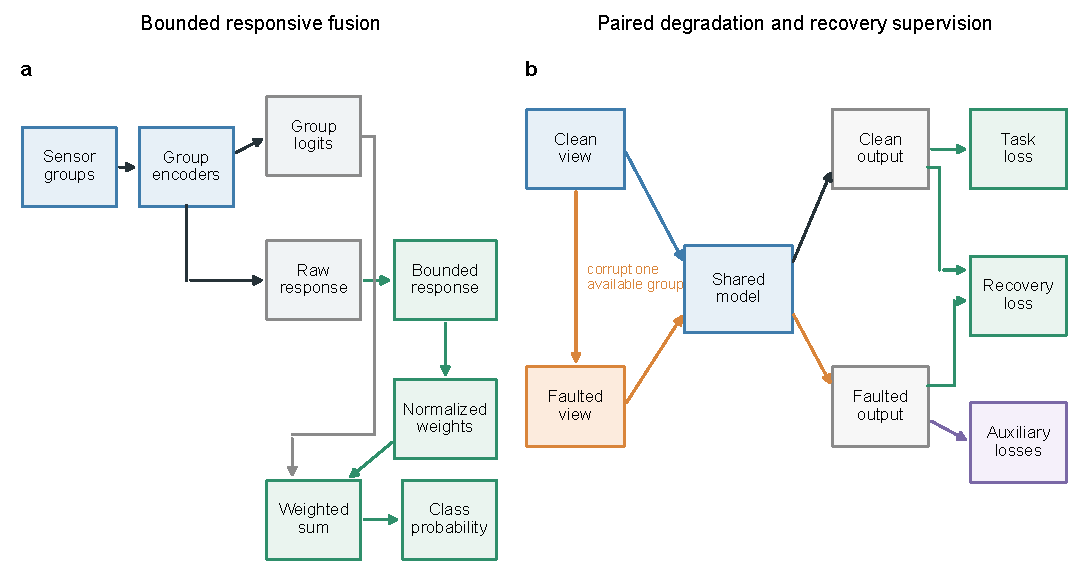
\includegraphics[width=\textwidth]{figure1_method_framework.pdf}
\caption{\textbf{Bounded responsive fusion and recovery supervision.} \textbf{a}, Each sensor group produces class logits and a bounded operational response. Availability, optional diagnostic quality and the response determine normalized fusion weights. Distinct connector ports separate the logit and weight contributions to the fused prediction. \textbf{b}, Clean and faulted views share model parameters. The detached clean prediction supervises recovery of the faulted prediction; proper-scoring and ranking terms are auxiliary controls.}
\label{fig:method}
\end{figure}
\FloatBarrier

\subsection{Comparators and mechanism ablations}

Early fusion concatenates zero-filled group features, masks and quality values before a $128\rightarrow64\rightarrow C$ multilayer perceptron. Uniform fusion averages group logits. EF-PD and UF-PD receive the same paired degradations and degraded-task loss as PDRF. The corruption-aware gated fusion model (CAGF) concatenates the four 32-dimensional group representations, masks and quality values, then applies a $64\rightarrow M$ softmax gate. It is the matched mixture-of-experts-style comparator: group classifiers act as experts and a sample-dependent unrestricted gate supplies their mixing coefficients. CAGF receives the same paired degradation, consistency and normalized-weight monotonicity losses. Direct weight ranking (DWR) adds a margin directly to the gate weight. The quality-only model uses $a_{im}q_{im}$ without a learned gate or bounded operational response.

To test whether a stronger interaction model alters the architecture comparison, RO-AT-GATE maps each physical sensor group to a 32-dimensional token, adds a learned group-identity embedding, and applies one four-head self-attention layer with a 64-unit feed-forward block. Unavailable groups are masked before attention. A shared $32+2\rightarrow16\rightarrow1$ head converts each contextualized token, availability flag and quality value into an unrestricted softmax gate. This compact attention baseline has 26,809 parameters, close to CAGF's 26,588, and receives exactly the same paired views and complete recovery objective as RO-CAGF. It is a sensor-group adaptation of modern cross-modal attention practice rather than a claim to reproduce a task-specific vision or language system \citep{li2024umdf,gao2024aleatoric,cho2025cocoon}.

The recovery-oriented multi-expert router (RO-MER) is a stronger sample-dependent control motivated by recent failure-resilient expert routing \citep{park2025mome}. Its candidate set contains one classifier from each physical group and one joint expert that maps all group representations, availability indicators and quality values through a $64$-unit hidden layer. A separate $64$-unit router produces a softmax distribution over the available group experts and the joint expert. For the shared monotonicity audit, the joint-expert probability is distributed uniformly over the groups available in that observation; this diagnostic allocation does not alter the fused prediction. RO-MER has 35,811 trainable parameters and receives the complete recovery objective and the same faults, batches, seeds and checkpoint rule as RO-CAGF and RO-PDRF-Full. It tests whether the conclusion survives a model that can switch between single-group evidence and explicit cross-group interaction, rather than merely changing the width of the original gate.

We additionally adapt Quality-aware Multimodal Fusion (QMF), originally evaluated for text--image classification and RGB--D scene recognition, to the same four sensor groups \citep{zhang2023qmf}. For group logits $\boldsymbol\mu_{im}$, the signed energy-derived quantity is $\bar c_{im}=\log\sum_c\exp(\mu_{imc})/10$. Because $\bar c_{im}$ can be negative, the implementation uses the positive confidence $c_{im}=\max(10^{-6},\bar c_{im})$ before fusing available-group logits as the unnormalized sum $\sum_m a_{im}\operatorname{stopgrad}(c_{im})\boldsymbol\mu_{im}$. The ranking loss uses cumulative per-sample cross-entropy histories to form normalized pairwise margins and enters at unit weight, matching the published implementation rule. Group encoders, paired corruption, optimizer, split and checkpoint criterion remain those of the present chemical experiment. We call this primary control QMF-PD. It aligns the decision, confidence-detachment and trajectory-ranking rules with the published code, but remains a sensor-group adaptation rather than an exact reproduction of the original backbones or tasks. Confidence scales, normalized versus unnormalized fusion, ranking weights and the previous adaptation are reported as sensitivity variants.

PDRF contains 19,740 trainable parameters on the chemical array, compared with 26,588 for CAGF and DWR, 35,811 for RO-MER, 26,182 for early fusion and 17,560 for uniform fusion. Ablations comprise paired degradation only (PD-ONLY), paired degradation plus normalized-weight monotonicity (PD-MONO), paired degradation plus response ranking (PD-RANK), the complete objective without $\mathcal L_{\mathrm{score}}$ (NO-LSCORE), and $\mathcal L_{\mathrm{score}}$ without $\mathcal L_{\mathrm{rank}}$ (LSCORE-NO-LRANK). A PDRF-NOQ model is trained and tested with all quality values fixed to one.

\subsection{Recovery-oriented extension}

The mechanism audit showed that reducing an affected group's weight was often necessary but not sufficient for prediction recovery. We therefore define recovery-oriented PDRF (RO-PDRF), which retains the PDRF architecture and adds recovery supervision. First, the degraded prediction is distilled from the detached clean-view prediction. Write $\widehat{\mathbf p}_i=\operatorname{stopgrad}(\mathbf p_i)$; then
\begin{equation}
\mathcal L_{\mathrm{rec}}=\frac{1}{|\mathcal V_{\mathcal B}|}
\sum_{i\in\mathcal V_{\mathcal B}}D_{\mathrm{KL}}\!\left[\widehat{\mathbf p}_i\,\|\,\mathbf p'_i\right].
\end{equation}
As with the removal consistency term, $\mathcal L_{\mathrm{rec}}$ is omitted when $\mathcal V_{\mathcal B}$ is empty.
This label-free teacher targets recovery of the clean class distribution instead of assuming that downweighting alone repairs the decision. We denote the base PDRF objective plus $0.30\mathcal L_{\mathrm{rec}}$ as RO-PDRF-Lite. Label-assisted best-view, affected-group-removal and confidence-selected teachers are evaluated only as sensitivity variants. Three additional teacher controls use the same principal split and fault: a hard 0.70 confidence threshold, continuous weighting and an exponential-moving-average (EMA) teacher \citep{tarvainen2017mean}. For continuous weighting, let $c_i=\max_c p_{ic}$ and $k_i=D_{\mathrm{KL}}[\operatorname{stopgrad}(\mathbf p_i)\,\|\,\mathbf p'_i]$. Then
\begin{equation}
\mathcal L_{\mathrm{rec,w}}=
\frac{\sum_{i\in\mathcal B}c_i k_i}
{\sum_{i\in\mathcal B}c_i+10^{-6}}.
\end{equation}
The EMA model is updated after every optimization step and only the student is used at inference. Decays 0.95, 0.99 and 0.995 are tested. To attenuate a single teacher's mistakes, clean/removal agreement (CRA) uses the mean of clean and affected-group-removal probabilities only when their predicted classes agree; student/EMA agreement (ECA) analogously averages the student-clean and EMA-clean probabilities only when their classes agree. The CE-conflict training audit retains recovery distillation when the clean-view cross-entropy does not exceed degraded-view cross-entropy. It uses training labels already present in the task losses, but the analogous conflict state is unavailable at test time; it is therefore a mechanistic diagnostic, not a deployable safeguard or fault selector. These controls were specified for the revision and do not redefine the principal comparison.

Second, multiclass Brier losses on clean and degraded predictions provide proper-scoring supervision,
\begin{equation}
\begin{aligned}
\mathcal L_{\mathrm{Brier}}={}&\frac{1}{|\mathcal B|}\sum_{i\in\mathcal B}\|\mathbf p_i-\mathbf e_{y_i}\|_2^2\\
&+\frac{1}{|\mathcal B|}\sum_{i\in\mathcal B}\|\mathbf p'_i-\mathbf e_{y_i}\|_2^2.
\end{aligned}
\end{equation}
The Brier term is the unweighted multiclass score averaged over observations; class weights are used for cross-entropy but are not inserted into the proper score. This preserves its standard probabilistic interpretation while classwise calibration is reported separately.
Third, a weak log barrier discourages boundary occupancy without removing the original finite quartic penalty. With $\epsilon=10^{-4}$, define $b_\epsilon(r)=-\log\{\max[\epsilon,1-(r/B)^2]\}$, $\bar b_{im}=b_\epsilon(r_{im})+b_\epsilon(r'_{im})$ and $Z_{\mathcal B}=\sum_{i\in\mathcal B}\sum_m a_{im}$. Its exact clean-plus-degraded implementation is
\begin{equation}
\mathcal L_{\mathrm{interior}}=Z_{\mathcal B}^{-1}
\sum_{i\in\mathcal B}\sum_m a_{im}\bar b_{im}.
\label{eq:interior}
\end{equation}
Unavailable groups are excluded by $a_{im}$; the clamp is solely a numerical safeguard near the open boundary. Fourth, a smooth one-versus-rest pairwise ranking loss directly supervises degraded-view class ordering. For class $c$, let $P_c$ and $N_c$ denote positive and negative observations in a minibatch, let $\mathcal C_{\mathcal B}=\{c:|P_c|>0,|N_c|>0\}$ be the eligible class set, and let $\phi_{ijc}=\operatorname{softplus}[-(\ell'_{ic}-\ell'_{jc})]$:
\begin{equation}
\begin{aligned}
\mathcal L_{\mathrm{AUC}}&=\frac{1}{|\mathcal C_{\mathcal B}|}\sum_{c\in\mathcal C_{\mathcal B}}A_c,\\
A_c&=\frac{\sum_{i\in P_c}\sum_{j\in N_c}\phi_{ijc}}{|P_c||N_c|}.
\end{aligned}
\label{eq:auc}
\end{equation}
Pairwise losses target class ordering directly rather than using cross-entropy as an indirect surrogate \citep{yang2021pairwise}. A class contributes only when the current minibatch contains at least one positive and one negative example; absent classes are skipped, and the pairwise term is omitted if no class is eligible. RO-PDRF-Full adds $0.30\mathcal L_{\mathrm{rec}}+0.05\mathcal L_{\mathrm{Brier}}+0.005\mathcal L_{\mathrm{interior}}+0.10\mathcal L_{\mathrm{AUC}}$ to Eq.~\eqref{eq:objective}. The formal hierarchy is fixed throughout: RO-PDRF-Lite is the primary practical model and software default; RO-PDRF-Full is the mechanistic full model used for complete-objective architecture comparisons; and RO-PDRF-EMA is a calibration-oriented sensitivity based on Full. The clean-view teacher is the formal specification because it removes label-assisted teacher selection without reducing affected-subset discrimination in the teacher audit. The test set is not used to fit model or ensemble parameters.

To separate recovery supervision from architecture, we also train recovery-oriented CAGF (RO-CAGF). It receives the same clean-view recovery distillation, Brier and degraded-view AUC losses as RO-PDRF-Full. Because an unrestricted softmax gate has no bounded operational response, its architecture-specific regularizer is a weak KL penalty from clean and degraded gates to the uniform distribution over available groups (weight 0.005), rather than the response-interior barrier used by RO-PDRF-Full. CAGF, RO-CAGF, PDRF and RO-PDRF-Full use identical data, fixed faults, seeds, minibatches, checkpoint rules and three training forward paths; each requires one inference path. We therefore call the design recovery-objective matched with architecture-specific regularization, rather than fully objective-symmetric. KL weights 0, 0.001, 0.005 and 0.020 and interior weights 0, 0.001, 0.005 and 0.020 are evaluated in a factorial sensitivity analysis. Additional controls apply clean-view distillation alone to early fusion, uniform fusion, CAGF and PDRF. A modality-dropout self-distillation baseline removes one available group per training pair, and a confidence-thresholded control applies distillation only when teacher confidence is at least 0.70. These controls test established consistency-training mechanisms rather than claiming a new divergence or distillation principle \citep{neverova2016moddrop,li2024umdf}.

\subsection{Calibration-only selective recovery}

Unconditional recovery can repair a wrong base prediction but can also overturn a correct one. We therefore evaluate two selective-recovery variants that choose between PDRF and RO-PDRF-Full for each observation. Batch~7 is divided chronologically into two disjoint halves. The first half fits one temperature for each model; the second half fits the selector and its threshold. On the selector half, four controlled fault mechanisms are generated with two calibration-only realizations each. Only observations for which the fault is actually applied to an available group enter selector fitting.

The selector receives neither the class label nor the fault type at inference. Its 12 inputs are base and recovery confidence, normalized entropy and their differences; Jensen--Shannon disagreement between the two predictions; disagreement of each prediction with the mean obtained by removing each available group in turn; agreement of their predicted classes with that leave-one-group-out consensus; and the fraction of legal group removals. A standardized logistic model is fitted only to calibration observations for which PDRF and RO-PDRF-Full differ in correctness, with the target indicating which model is correct. Candidate thresholds from 0.50 to 0.90 are then evaluated on the complete selector half. SR-PDRF-Balanced maximizes calibration accuracy and breaks ties by lower negative transfer. SR-PDRF-Safe first minimizes the rate at which selection retains an RO-PDRF-Full error when PDRF is correct, then maximizes accuracy and recovery. At test time, RO-PDRF-Full is used only when the frozen selector probability exceeds the corresponding threshold; otherwise the system falls back to PDRF. No held-out observation, label or metric is used to fit temperatures, selector coefficients or thresholds. The inference audit includes two ordinary model passes and four leave-one-group-out recovery passes; selective recovery is therefore a safety-oriented layer rather than a free computational improvement.

\subsection{Chemical-sensor dataset and fixed faults}

The UCI Gas Sensor Array Drift Dataset contains 13,910 observations from 16 metal-oxide sensors, six gas classes and 10 acquisition batches over 36 months \citep{vergara2012dataset,vergara2012drift}. Each sensor contributes eight extracted response features. The principal grouping uses four consecutive sensors per group. All models receive the same grouping. Sensitivity analyses additionally use interleaved and five fixed random partitions; no partition is called a physical modality.

Batches 1--6 train the models. The first 60\% of batch 7 selects checkpoints, and the remaining 40\% is reserved for calibration; the selective-recovery experiment further divides that calibration partition into temperature and selector halves. Batches 8--10 are held out for testing. The primary controlled fault assigns 40\% of test observations a standardized Gaussian intervention of scale 3 on group 1 and leaves $q=1$. We call an intervention silent when the corrupted group is available without a quality alert, that is, $a_{im^*}=1$ and $q_{im^*}=1$. Fault assignment and missingness are sampled independently. Of 4,364 test observations, 1,765 are assigned the principal fault; group~1 remains available and receives a nonzero intervention in 1,436, whereas it is masked in the remaining 329. The strict recovery estimand is the former \emph{fault-applied-and-available} subset. The full assignment subset is reported only as a sensitivity analysis because an assigned but masked group cannot transmit the intervention. Twenty percent random group missingness is applied to controlled-fault test views. Fault indices, missingness masks and intervention values are fixed across methods and optimization seeds.

Checkpoint selection and temperature calibration use separate fault-free views with independently generated 10\% group missingness; no controlled Gaussian, offset, drift or stuck-at intervention is added to either subset. The checkpoint criterion is unweighted cross-entropy on the complete selection subset. Temperature is fitted on all calibration observations, not an affected subset, by minimizing unweighted multiclass negative log-likelihood. The resulting scalar is specific to each fitted seed and method and is then applied unchanged to clean, affected-assignment and unaffected test observations under every controlled fault. The 20\% missingness rate is used only for controlled-fault test views; training, selection and calibration use 10\%, and the natural no-fault chemical view uses no imposed test missingness.

The expanded fault study crosses four prespecified mechanisms with realizations 70001--70008 and fitted seeds 101--105. Model fitting always uses the Gaussian paired degradation defined above; offset, drift and stuck-at are test-time interventions only. Gaussian faults add independent standardized noise. Offset faults add a scale-3 featurewise signed displacement. Drift uses the same signed displacement multiplied by a monotone 0.25--1.00 trajectory over held-out acquisition order. Stuck-at faults replace the affected group's standardized features by a signed scale-3 vector. Within each realization, all four mechanisms share affected rows and group-missingness masks, while intervention-specific values remain fixed across methods. These are controlled repeats on the same instrument. Additional exploratory interventions vary prevalence (0.10, 0.40, 0.70), scale (1, 3, 5), sensor group, gain, clipping and dual-group corruption.

Quality controls include reported $q$, row-shuffled $q$, misleading $q$, absent $q$, training without $q$ and a quality-only comparator. Leave-one-group-out training assigns zero degradation probability to each group in turn before testing that group's fault. Hyperparameter sensitivity varies $B\in\{1,2,3,4,5\}$, $\beta\in\{0.10,0.25,0.50,0.75\}$ and ranking weight $\in\{0.05,0.15,0.30\}$. The recovery-objective-matched stress grid contains 17 conditions spanning fault type, affected group, severity and prevalence; these conditions share observations and fitted models and are not treated as 17 independent replications. These sensitivity analyses are exploratory and are not used to replace the prespecified main setting.

\subsection{Independent hydraulic test-rig validation}

The UCI Condition Monitoring of Hydraulic Systems dataset contains 2,205 raw 60-s cycles from an experimental hydraulic rig and native condition labels for cooler, valve, pump and accumulator states (DOI: \href{https://doi.org/10.24432/C5CW21}{10.24432/C5CW21}) \citep{helwig2018hydraulic,helwig2015condition}. We retain 1,449 cycles marked as stable. Fourteen physical sensors form five groups by measured quantity: six pressure sensors, two flow sensors, four temperature sensors, motor power and vibration. This grouping is defined before model fitting and follows the measurement system rather than a random partition.

For each sensor, we calculate mean, standard deviation, minimum, maximum, quartiles, root-mean-square value and linear slope. Physical groups contain different numbers of sensors and therefore different summary-vector lengths. The principal representation linearly resamples each flattened group vector to 48 positions so all groups can use the same encoder architecture and parameter budget. This operation is a dimensional alignment convention, not temporal interpolation; it may nevertheless smooth adjacent summary coordinates or alter their relative spacing. A no-interpolation audit therefore places each native summary vector at the start of a 48-position vector and zero-pads only the unused tail. Each component task first uses a fixed stratified 60/15/10/15\% split. A stricter audit preserves acquisition order within every native condition class, assigns contiguous 60/15/10/15\% blocks and discards five guard cycles at each split boundary. A single global chronological split is invalid because cooler and accumulator states occupy non-overlapping acquisition ranges and would leave unseen classes in training or test. PDRF-NOQ, RO-PDRF-Full-NOQ and CAGF are fitted with five matched seeds for both representations; recovery-objective-matched RO-PDRF-Full and RO-CAGF are refitted under the guarded blocked split. Pressure-group and vibration-group faults affect the same 40\% of test cycles across methods. Component-condition labels are native to the test-rig experiment; sensor faults remain controlled interventions. Related hydraulic work is used only for context, not as a directly reproduced architecture \citep{ma2021multirate,keleko2023hydraulic,yildirim2025hydraulic}.

\subsection{Real-operational AHU sensor-fault validation}

We additionally use the open real-operational AHU dataset from an auditorium, a hospital and a large office (Figshare DOI: \href{https://doi.org/10.6084/m9.figshare.27147678.v3}{10.6084/m9.figshare.27147678.v3}) \citep{wang2025ahuoperational,wang2024ahudataset}. It contains hourly building-management-system records collected for one year per building. Four HVAC specialists with at least 20 years of experience annotated operating conditions, and two additional experts cross-checked a random subset. The present binary task retains normal operation and the native return- or supply-air temperature sensor-fault labels. No artificial corruption is applied to any AHU test record. Crucially, the public labels identify the sensor fault itself; they do not provide an independent component-condition, energy or control target to be recovered after suppressing that sensor. AHU direct diagnosis is therefore intentionally designated a negative task-boundary experiment, not a third validation of downstream recovery.

Seven harmonized measurements form five physically interpretable groups. Each building uses a chronological 60\%/15\%/10\%/15\% split, untouched future-time testing and five matched seeds. A leave-one-building-out audit trains on two buildings and holds out the third; the main text retains only the task boundary, within-building comparison and hospital transfer collapse. Full grouping, temporal controls, feature-shift, reversal, GroupDRO, unlabeled-target adaptation, risk--coverage and conformal specifications are reported in the Supplementary Information \citep{sun2016coral,sagawa2020groupdro,mirza2022normalization,podkopaev2021distribution}.

\subsection{Training, metrics and statistical analysis}

AdamW uses learning rate $2\times10^{-3}$, weight decay $10^{-4}$, batch size 256 and gradient clipping at 5. Chemical-array training uses at most 60 epochs, hydraulic training uses at most 80 and AHU training uses at most 12. Checkpoints minimize unweighted selection cross-entropy and stop after nine epochs without an improvement greater than $10^{-4}$. RO-PDRF-Lite, RO-PDRF-Full, RO-PDRF-EMA and all teacher controls use this identical criterion; no test metric selects a checkpoint or variant. Class weights are $n/(Cn_c)$. No dropout or batch normalization is used.

Parameter counts and wall-clock costs are audited on the same CPU-only PyTorch runtime. Timings exclude data download and preprocessing, use identical test observations and are descriptive rather than hardware-independent complexity guarantees. Linear-layer multiply--accumulate operations, corresponding floating-point operations, model-state bytes and forward-activation bytes are counted for 2, 4, 8 and 16 sensor groups. Training loss, checkpoint cross-entropy and pre-clipping gradient norms are recorded by epoch for the consistency controls.

We report accuracy, macro-F1, macro-AUROC, macro/micro-AUPRC, NLL, multiclass Brier score, per-class precision, recall, F1, AUROC and AUPRC, confusion matrices and ECE with 10, 15, 20 fixed-width bins and 15 equal-frequency bins. Temperature scaling is fitted separately for every seed. The revised headline endpoint is macro-AUROC on the strict fault-applied-and-available subset under the fixed silent-Gaussian fault (seed 70001). The four-method comparison uses 10 matched optimization seeds; the assignment-only subset is a protocol sensitivity. Exact two-sided Wilcoxon signed-rank tests and seed intervals describe fitting stability, not population-level or device-level replication. Because the strict estimand, selector and multi-expert baseline were added after reviewer-driven audit of earlier results, their $P$ values are not labelled preregistered confirmatory evidence. Fault-realization, fault-type, hydraulic, AHU, calibration, ensemble, teacher and sensitivity analyses are likewise interpreted at their stated exploratory evidence levels. An earlier recovery/calibration run and a superseded factorial rerun used a label-assisted teacher or a different fixed fault instance; both are confined to protocol sensitivity in the Supplementary Information. A post-hoc non-inferiority margin appears only as a descriptive supplementary analysis.

Paired seed differences quantify repeated fitting and are not interpreted as external replication. The Gaussian analysis resamples fault realizations and crossed optimization-seed clusters. The four-mechanism analysis resamples fault type and shares each sampled optimization-seed cluster across fault cells because one fitted model is evaluated under every intervention; with only four top-level mechanisms, these intervals are descriptive. Each bootstrap uses 5,000 replicates, and all reported intervals are equal-tailed percentile intervals. Batch-stratified summaries retain batches 8--10 as acquisition clusters. For the fixed 10-model strict-subset ensemble, a two-stage paired bootstrap first resamples acquisition batch and then observations within batch. It quantifies this fitted ensemble and test sample, not retraining or new devices. The 17 sensor-group, fault-type, severity and prevalence conditions remain correlated stress tests because they reuse observations and fitted models. Hydraulic summaries report condition effect sizes, median and range, leave-one-task-out means and a task--fault--seed hierarchical bootstrap; no condition-level value is interpreted as device-level replication. AHU results remain building-specific. Exact McNemar testing compares ensemble correctness. Formal and exploratory analyses are identified in the source metadata.

\begin{figure}[ht]
\centering
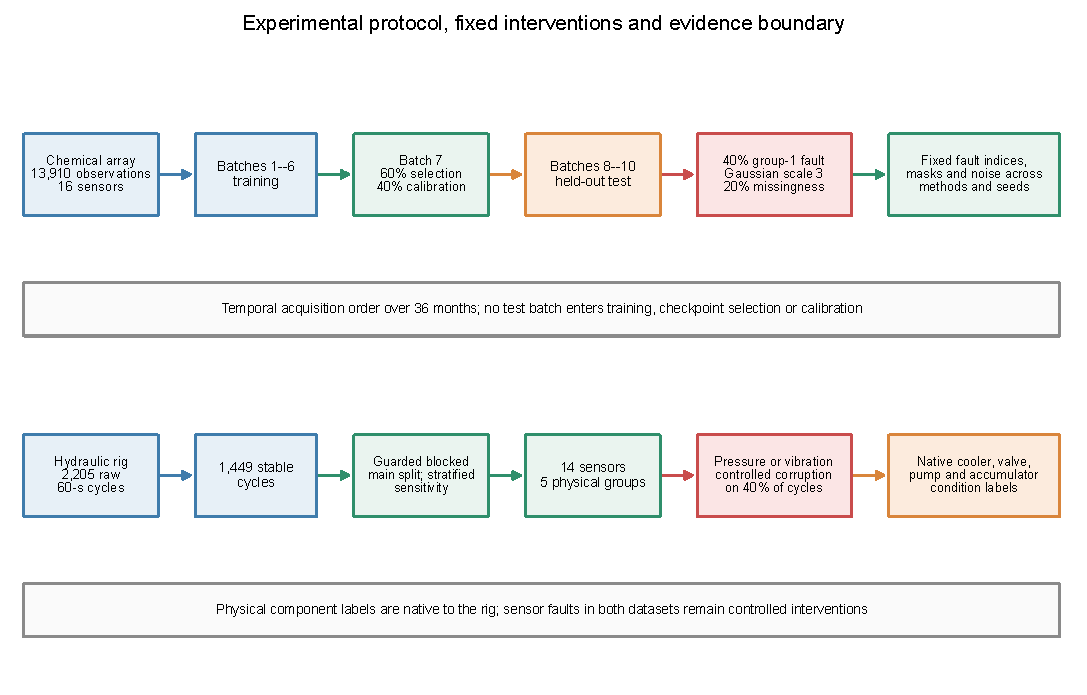
\includegraphics[width=\textwidth]{figure2_experimental_protocol.pdf}
\caption{\textbf{Integrated experimental protocol and controlled fault design.} The upper lane follows the chemical-array acquisition order from batches 1--6 training through Batch~7 checkpoint selection/calibration to held-out batches 8--10; fault indices, masks and intervention values are fixed across methods and seeds. The lower lane follows the independent hydraulic rig from stable 60-s cycles to the guarded within-condition blocked main analysis; the earlier stratified split is retained only as a sensitivity analysis. Component-condition labels are native to the rig, whereas chemical, pressure and vibration sensor corruptions remain controlled interventions.}
\label{fig:protocol}
\end{figure}
\FloatBarrier

\section{Results}

\subsection{The strict applied-fault estimand isolated recovery from assignment}

The fault generator assigned group~1 corruption to 1,765 held-out observations, but independent missingness masked that group in 329. The strict analysis therefore contains the 1,436 observations on which a nonzero intervention reached an available group. Mean macro-AUROC across 10 matched fits was 0.7865 for CAGF, 0.7941 for RO-CAGF, 0.7804 for PDRF and 0.7960 for RO-PDRF-Full. Recovery supervision improved the bounded model by 0.0156 in all 10 fits (exact $P=0.0020$; Table~\ref{tab:major9-strict}). It improved the unrestricted gate by 0.0077 in six of 10 fits ($P=0.3223$). The recovery-matched RO-PDRF-Full--RO-CAGF contrast was only $+0.0018$, with four of 10 positive differences and $P=0.8457$. Thus the strict result supports recovery supervision but does not support superiority of the bounded architecture.

Aggregation reinforced this distinction. For the fixed 10-model probability ensemble, a batch-to-observation bootstrap estimated RO-PDRF-Full--PDRF as $+0.0145$ (95\% interval $+0.0087$ to $+0.0268$), whereas RO-PDRF-Full--RO-CAGF was $-0.0168$ ($-0.0296$ to $+0.0066$). These intervals condition on the fitted models and the three held-out acquisition batches; they are not retraining or device-replication intervals.

\begin{table}[ht]
\centering
\caption{Strict fault-applied-and-available macro-AUROC effects under the fixed chemical Gaussian intervention. Differences are paired across 10 optimization seeds. Exact Wilcoxon tests describe fitting stability and are not interpreted as independent-device inference.}
\label{tab:major9-strict}
\resizebox{0.78\textwidth}{!}{\begin{tabular}{lrrrr}
\toprule
Contrast & Mean $\Delta$ AUROC & SD & Wins/10 & $P$ \\
\midrule
RO-PDRF - PDRF & +0.0156 & 0.0047 & 10/10 & 0.0020 \\
RO-PDRF - RO-CAGF & +0.0018 & 0.0203 & 4/10 & 0.8457 \\
\bottomrule
\end{tabular}}
\end{table}

\subsection{Assignment-based sensitivity explained the earlier architecture contrast}

On all 1,765 fault-assigned rows, including rows on which group~1 was masked, CAGF, RO-CAGF, PDRF and RO-PDRF-Full achieved macro-AUROC 0.792, 0.797, 0.791 and 0.804, respectively (Table~\ref{tab:major3-chemical}). The recovery effects remained positive, but the recovery-matched architecture difference increased from $+0.0018$ on the strict subset to $+0.0073$. On the 329 assigned-but-unavailable rows alone, this architecture contrast was $+0.0337$ even though the fault could not enter the prediction. The assignment estimand therefore mixed fault recovery with ordinary missing-group behavior and inflated the apparent architecture separation. It is retained for reconciliation with earlier analyses, not as the headline endpoint.

The stress grid tested whether this conclusion depended on the main corruption. RO-PDRF-Full exceeded RO-CAGF in 14 of 17 conditions, with a descriptive mean affected-AUROC difference of 0.0159. RO-PDRF-Full exceeded PDRF and RO-CAGF exceeded CAGF in all 17. These are robustness summaries, not independent hypothesis tests, because the conditions reuse observations and fitted models. The post-hoc non-inferiority calculation is confined to the Supplementary Information and is not part of the main evidence chain.

Architecture-specific regularization did not reverse the chemical contrast: RO-PDRF-Full had the higher mean in all 16 KL/interior combinations, although no individual 10-seed contrast reached $P<0.05$; the full grid is reported in the Supplementary Information.

\begin{table}[ht]
\centering
\caption{Assignment-defined chemical-array sensitivity analysis. Values are means across 10 matched seeds and include 329 rows on which the assigned group was unavailable. CAGF/PDRF denotes architecture and RO denotes recovery-oriented training. The strict fault-applied result is reported in Table~\ref{tab:major9-strict}.}
\label{tab:major3-chemical}
\resizebox{0.86\textwidth}{!}{\begin{tabular}{lrrrrr}
\toprule
Method & All AUROC & Aff. AUROC & Aff. AUPRC & Aff. NLL & Aff. ECE \\
\midrule
CAGF & 0.817 & 0.792 & 0.505 & 2.095 & 0.277 \\
RO-CAGF & 0.819 & 0.797 & 0.512 & 2.071 & 0.275 \\
PDRF & 0.834 & 0.791 & 0.509 & 3.085 & 0.369 \\
RO-PDRF-Full & 0.840 & 0.804 & 0.525 & 2.650 & 0.342 \\
\bottomrule
\end{tabular}}
\end{table}

\subsection{Clean-view distillation accounted for most of the recovery gain}

The objective ladder separated the established consistency mechanism from the auxiliary terms. Adding clean-view distillation to paired-degradation training increased affected macro-AUROC from 0.747 to 0.758 for early fusion and from 0.763 to 0.791 for uniform fusion (both 10 matched seeds; $P=0.0020$ and $P=0.0039$). The same addition increased CAGF from 0.792 to 0.800 and PDRF from 0.791 to 0.802. RO-PDRF-Full reached 0.804, only 0.002 above RO-PDRF-Lite; the paired contrast was not significant ($P=0.1934$). RO-PDRF-Lite trained in $9.2\pm2.7$~s versus $22.7\pm5.6$~s for Full across the same 10 CPU runs, with identical parameters and one inference pass. Lite was therefore neither uniformly inferior nor uniformly superior to Full: Full had a small descriptive ranking advantage, whereas Lite had the lower measured training cost. Lite remains the primary practical model and software default when recovery ranking and cost are considered jointly; Full is retained for mechanistic analysis, and EMA is the calibration-oriented sensitivity when improved probability quality justifies additional training complexity.

A principle-matched modality-dropout/self-distillation control reached 0.703 affected AUROC, below early fusion with Gaussian paired degradation and clean distillation (0.758). Predictive-entropy fusion reached 0.754. The parameter-matched attention gate reached 0.784 under the complete recovery objective, compared with 0.797 for RO-CAGF and 0.804 for RO-PDRF-Full. Within the unified sensor-group protocol, the official-rule-aligned QMF-PD adaptation reached 0.775 across 10 seeds, with clean matched-mask AUROC 0.845, affected NLL 2.514 and ECE 0.287. The concise sensitivity table in the Supplementary Information shows affected AUROC 0.742--0.768 as confidence scale, fusion normalization and ranking weight changed, while clean AUROC remained 0.840--0.847. Thus, the adapted QMF-style energy-confidence rule did not reach RO-PDRF-Full affected ranking in this protocol. This comparison does not establish general superiority over QMF because the common sensor encoders, paired corruption and chemical task do not reproduce its original task-specific backbones.

Confidence-thresholding at 0.70 changed PDRF clean-distillation AUROC from 0.802 to 0.801, continuous confidence weighting gave 0.801, and an EMA teacher gave 0.803. None differed significantly from ordinary clean distillation. With the complete recovery objective, RO-PDRF-EMA increased affected AUROC from 0.8043 to 0.8059 ($P=0.2324$), while reducing NLL from 2.650 to 2.413 and ECE from 0.342 to 0.321. CRA and ECA reached affected AUROC 0.803 and 0.805, respectively. The CE-conflict training audit reached 0.806, but its conditional error-transfer rate remained 35.7\%. These variants are teacher-error audits rather than new headline models.

\begin{table}[ht]
\centering
\caption{Consistency-training ladder under the unique chemical headline fault. Values are means across 10 matched optimization seeds. Differences and 95\% intervals are paired against clean distillation within architecture; $P$ values are exact two-sided Wilcoxon tests.}
\label{tab:major5-ladder}
\resizebox{\textwidth}{!}{\begin{tabular}{llrrr}
\toprule
Architecture & Model/training condition & Affected AUROC & $\Delta$ vs clean distillation (95\% CI) & $P$ \\
\midrule
EF-PD & EF-PD & 0.747 $\pm$ 0.006 & -0.012 [-0.016, -0.007] & 0.0020 \\
EF-PD & EF-PD + clean distillation & 0.758 $\pm$ 0.006 & Reference & -- \\
UF-PD & UF-PD & 0.763 $\pm$ 0.010 & -0.027 [-0.036, -0.018] & 0.0039 \\
UF-PD & UF-PD + clean distillation & 0.791 $\pm$ 0.008 & Reference & -- \\
CAGF & CAGF & 0.792 $\pm$ 0.027 & -0.009 [-0.023, +0.006] & 0.2754 \\
CAGF & CAGF + clean distillation & 0.800 $\pm$ 0.024 & Reference & -- \\
CAGF & RO-CAGF & 0.797 $\pm$ 0.022 & -0.003 [-0.012, +0.006] & 0.6250 \\
PDRF & PDRF & 0.791 $\pm$ 0.010 & -0.012 [-0.014, -0.009] & 0.0020 \\
PDRF & RO-PDRF-Lite & 0.802 $\pm$ 0.008 & Reference & -- \\
PDRF & RO-PDRF-Full & 0.804 $\pm$ 0.009 & +0.002 [-0.001, +0.005] & 0.1934 \\
\bottomrule
\end{tabular}}
\end{table}

\begin{table}[ht]
\centering
\caption{Published/adapted baselines and teacher controls under the principal chemical fault. Values are affected-subset means across 10 matched seeds after temperature scaling. Role distinguishes comparison baselines, the practical default, mechanistic Full model, calibration sensitivity and diagnostic audits. Lite adds clean recovery distillation; Full also adds Brier, ranking and response-interior terms. CRA and ECA are agreement controls; CE-conflict is label-assisted and training-only. Lower NLL, Brier and ECE are better.}
\label{tab:major7-controls}
\resizebox{\textwidth}{!}{\begin{tabular}{lp{0.17\textwidth}rrrrrr}
\toprule
Method & Role & Parameters & Seeds & Affected AUROC & NLL & Brier & ECE \\
\midrule
QMF-PD & Published-method adaptation & 17,560 & 10 & 0.775 & 2.514 & 0.792 & 0.287 \\
RO-AT-GATE & Strong learned baseline & 26,809 & 10 & 0.784 & 1.826 & 0.736 & 0.210 \\
RO-CAGF & Architecture-matched baseline & 26,588 & 10 & 0.797 & 2.071 & 0.770 & 0.275 \\
RO-PDRF-Lite & Practical default & 19,740 & 10 & 0.802 & 2.717 & 0.809 & 0.342 \\
RO-PDRF-Full & Mechanistic full model & 19,740 & 10 & 0.804 & 2.650 & 0.809 & 0.342 \\
RO-PDRF-EMA & Calibration sensitivity & 19,740 & 10 & 0.806 & 2.413 & 0.792 & 0.321 \\
RO-PDRF-Full-CRA & Diagnostic audit & 19,740 & 10 & 0.803 & 2.730 & 0.819 & 0.349 \\
RO-PDRF-Full-ECA & Diagnostic audit & 19,740 & 10 & 0.805 & 2.494 & 0.804 & 0.332 \\
CE-conflict training audit & Diagnostic audit & 19,740 & 10 & 0.806 & 2.592 & 0.801 & 0.336 \\
\bottomrule
\end{tabular}}
\end{table}

Eight independently generated, method-shared fault realizations then separated corruption variability from optimization variability. RO-PDRF-Full exceeded RO-CAGF in all eight realization means, with mean difference $+0.0123$ and a hierarchical 95\% interval of $+0.0054$ to $+0.0189$. Recovery gains were positive for both PDRF ($+0.0118$, interval $+0.0104$ to $+0.0130$) and CAGF ($+0.0112$, interval $+0.0064$ to $+0.0160$). Batch-specific RO-PDRF-Full--RO-CAGF means were $+0.0175$, $+0.0149$ and $+0.0101$ for batches 8, 9 and 10; 22 of 24 batch--realization means were positive. These are repeated corruptions of one instrument, not independent devices, but they move the principal inference above the optimization-seed level.

The expanded design crossed Gaussian, offset, acquisition-ordered drift and stuck-at corruption with eight realizations and five fitted seeds. RO-PDRF-Full affected AUROC was 0.803, 0.816, 0.826 and 0.811, compared with 0.792, 0.786, 0.791 and 0.778 for RO-CAGF. Per-fault RO-PDRF-Full--RO-CAGF effects were $+0.011$ (95\% interval $-0.009$ to $+0.028$), $+0.030$ ($+0.003$ to $+0.057$), $+0.035$ ($+0.012$ to $+0.057$) and $+0.034$ ($+0.003$ to $+0.062$), respectively. The four-type aggregate was $+0.027$ ($+0.002$ to $+0.051$), but is descriptive because only four top-level fault clusters exist. Leave-one-fault-type-out means remained positive ($+0.025$ to $+0.033$), with one interval crossing zero. RO-PDRF-EMA with decay 0.99 reduced NLL by 0.283 and ECE by 0.0228 across the same design, while its AUROC interval crossed zero. These repeats remain controlled interventions on one instrument, not natural hardware-failure or device replication.

\begin{figure}[p]
\centering
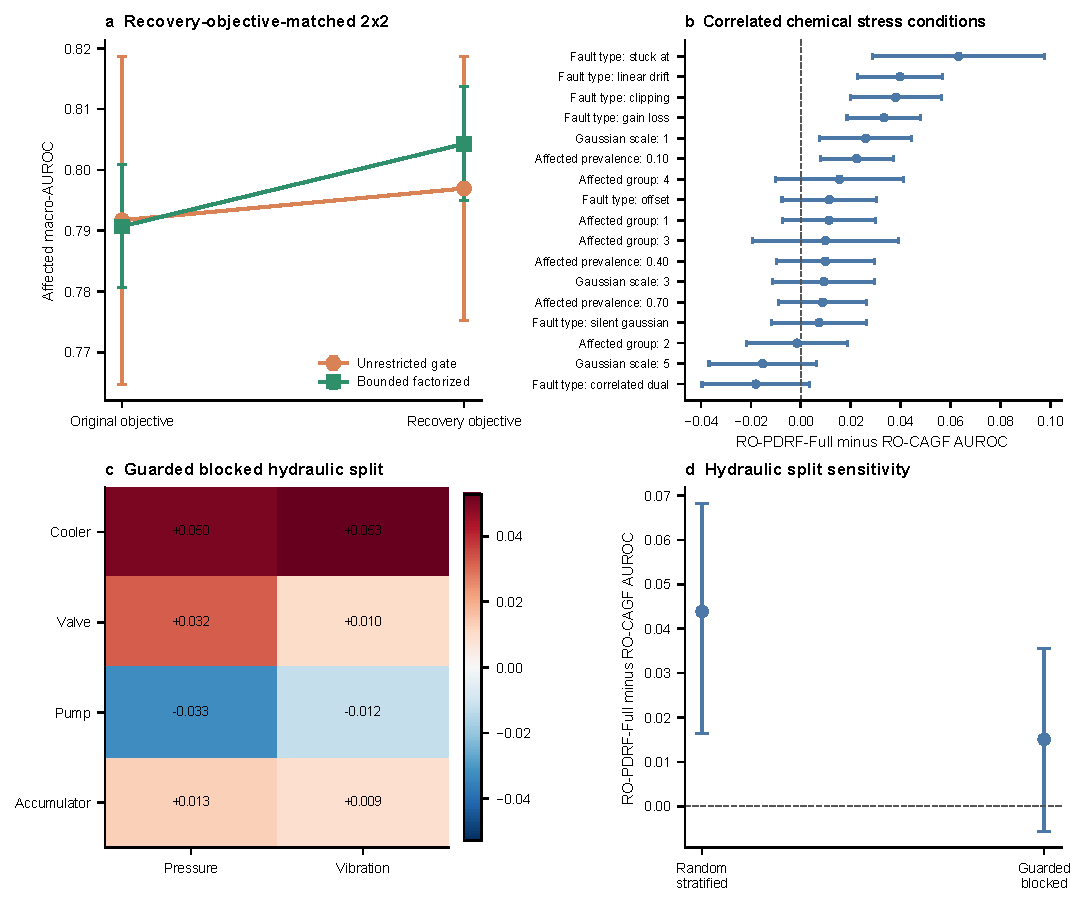
\includegraphics[width=\textwidth]{figure7_objective_matched.pdf}
\caption{\textbf{Recovery-objective and architecture comparison.} \textbf{a}, Chemical-array $2\times2$ comparison for affected macro-AUROC; the bounded recovery endpoint is RO-PDRF-Full. \textbf{b}, RO-PDRF-Full--RO-CAGF differences across 17 correlated chemical stress conditions; error bars show seed standard deviations and are descriptive. \textbf{c}, hydraulic differences under the guarded within-condition blocked split across four native component tasks and two controlled fault groups from one rig. \textbf{d}, random-stratified versus guarded-blocked hydraulic differences. Intervals are paired bootstrap intervals over the stated unit.}
\label{fig:objective-matched}
\end{figure}
\FloatBarrier

\subsection{A stronger expert router did not remove the bounded model's advantage}

RO-MER strengthened the unrestricted-gating comparison without relying on the original CAGF parameterization (Table~\ref{tab:major9-modern}). It exceeded RO-CAGF for offset, drift and stuck-at corruption, but not for Gaussian noise. Across the four controlled mechanisms, RO-MER--RO-CAGF was $+0.0095$ with a descriptive crossed-factor interval of $-0.0043$ to $+0.0215$. RO-PDRF-Full exceeded RO-MER for every mechanism and by $+0.0154$ on average (descriptive interval $+0.0106$ to $+0.0206$). Mean CPU training times were 12.1, 11.8 and 18.6~s for RO-CAGF, RO-MER and RO-PDRF-Full, respectively, with 26,588, 35,811 and 19,740 parameters. The result survives a stronger interaction baseline in this controlled instrument, but four fault types and one instrument do not establish universal architectural superiority.

\begin{table}[ht]
\centering
\caption{Strict fault-applied-and-available macro-AUROC for the recovery-oriented gate, multi-expert router and complete bounded model. Values are means $\pm$ standard deviations across 10 matched optimization seeds.}
\label{tab:major9-modern}
\resizebox{0.82\textwidth}{!}{\begin{tabular}{lrrr}
\toprule
Fault & RO-CAGF & RO-MER & RO-PDRF-Full \\
\midrule
gaussian & 0.795 $\pm$ 0.023 & 0.787 $\pm$ 0.012 & 0.799 $\pm$ 0.010 \\
offset & 0.792 $\pm$ 0.029 & 0.807 $\pm$ 0.011 & 0.822 $\pm$ 0.013 \\
drift & 0.799 $\pm$ 0.025 & 0.813 $\pm$ 0.014 & 0.829 $\pm$ 0.013 \\
stuck-at & 0.780 $\pm$ 0.038 & 0.797 $\pm$ 0.016 & 0.815 $\pm$ 0.011 \\
\bottomrule
\end{tabular}}
\end{table}

\subsection{Calibration-only fallback prevented most negative transfer}

The selective-recovery layer converted the teacher-error audit into an inference-time decision. Across four mechanisms and 10 fitted model pairs, the strict test set produced 1,692 recovery opportunities, in which PDRF was wrong and RO-PDRF-Full was correct, and 1,375 negative-transfer opportunities with the opposite ordering. SR-PDRF-Balanced preserved 569 recoveries (33.6\%) and left 294 negative transfers (21.4\%), preventing 78.6\% of the avoidable losses. SR-PDRF-Safe preserved 303 recoveries (17.9\%) and left 137 negative transfers (10.0\%), preventing 90.0\%. It selected the recovery model for 49.2\% of evaluated predictions, compared with 64.5\% for Balanced. Counts pool repeated predictions across 10 optimization seeds and four controlled fault mechanisms and therefore quantify selector behavior, not 57,440 independent physical events.

The safety gain had a measurable ranking cost (Table~\ref{tab:major9-safe}). Averaged descriptively over the four mechanisms, SR-PDRF-Safe was $+0.0042$ above PDRF (interval $+0.0021$ to $+0.0066$) and $-0.0005$ below unconditional RO-PDRF-Full ($-0.0052$ to $+0.0036$). Under the principal Gaussian fault, Safe gave 0.792 macro-AUROC versus 0.799 for Full and 0.784 for PDRF. Safe therefore protects base-model corrections rather than dominating unconditional recovery. Figure~\ref{fig:major9-upgrade} links the strict estimand, architecture control and this safety--recovery trade-off.

\begin{table}[ht]
\centering
\caption{Calibration-only selective recovery on the strict fault-applied-and-available subset. Values are macro-AUROC means $\pm$ standard deviations across 10 matched optimization seeds. Balanced prioritizes calibration accuracy; Safe prioritizes lower calibration negative transfer.}
\label{tab:major9-safe}
\resizebox{0.96\textwidth}{!}{\begin{tabular}{lrrrr}
\toprule
Fault & PDRF & RO-PDRF-Full & SR-PDRF-Balanced & SR-PDRF-Safe \\
\midrule
gaussian & 0.784 $\pm$ 0.011 & 0.799 $\pm$ 0.010 & 0.794 $\pm$ 0.011 & 0.792 $\pm$ 0.011 \\
offset & 0.821 $\pm$ 0.014 & 0.822 $\pm$ 0.013 & 0.824 $\pm$ 0.012 & 0.824 $\pm$ 0.012 \\
drift & 0.829 $\pm$ 0.014 & 0.829 $\pm$ 0.014 & 0.831 $\pm$ 0.013 & 0.832 $\pm$ 0.013 \\
stuck-at & 0.812 $\pm$ 0.011 & 0.815 $\pm$ 0.011 & 0.815 $\pm$ 0.009 & 0.816 $\pm$ 0.009 \\
\bottomrule
\end{tabular}}
\end{table}

\begin{figure}[p]
\centering
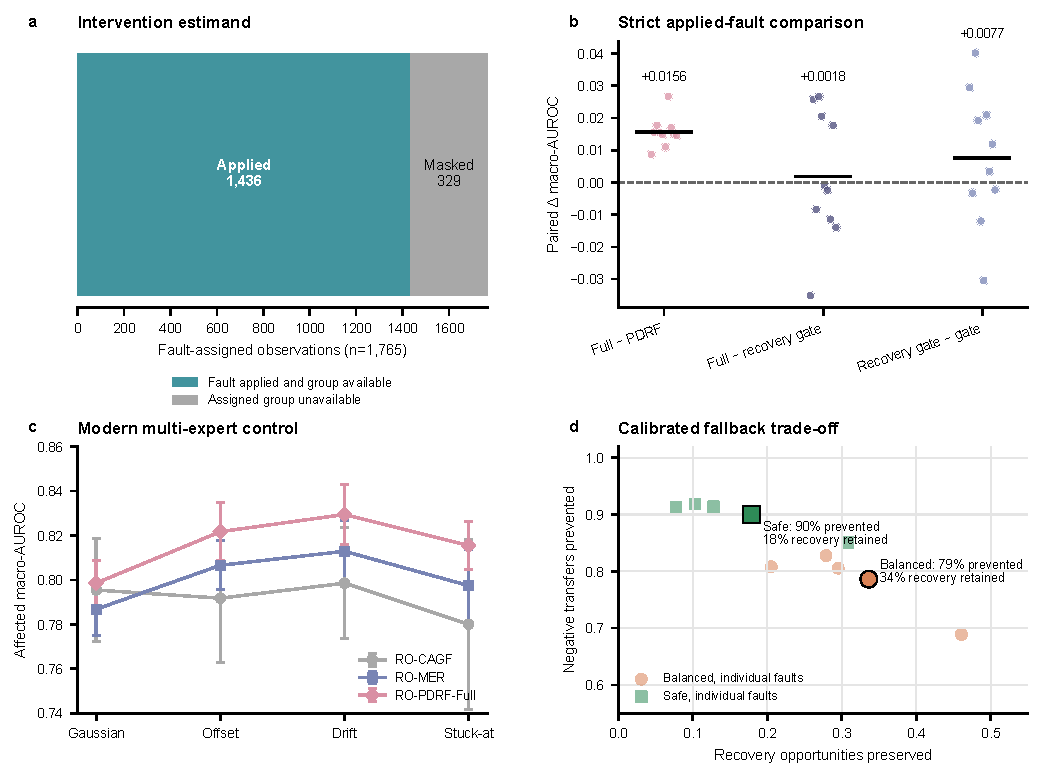
\includegraphics[width=\textwidth]{figure8_strict_safe_upgrade.pdf}
\caption{\textbf{Strict recovery evidence and calibration-only fallback.} \textbf{a}, Test-set accounting separates fault assignment from a nonzero intervention on an available group. \textbf{b}, paired 10-seed macro-AUROC effects on the strict Gaussian subset; seed variation reflects repeated optimization only. \textbf{c}, recovery-oriented multi-expert routing strengthens the gated comparator across four controlled mechanisms. \textbf{d}, selection trades retained recovery opportunities against remaining negative transfer. Balanced and Safe thresholds are fitted on Batch~7 only; points use the strict held-out test subset.}
\label{fig:major9-upgrade}
\end{figure}
\FloatBarrier

\subsection{Downweighting remained distinct from prediction recovery}

In the clean-teacher headline run, the affected group's normalized weight decreased in 80.2\% of affected predictions, yet 41.9\% of all affected predictions still failed despite that decrease. Recovery distillation was the largest leave-one-loss-out contribution ($+0.0105$ affected AUROC; 10/10 seeds, $P=0.0020$). Brier supervision contributed $+0.0018$ ($P=0.0098$), degraded-AUC supervision $+0.0023$ ($P=0.0645$), and the response-interior term $+0.0008$ ($P=0.2754$). The clean, label-assisted best-view, removal and confidence-selected teachers produced near-identical sensitivity results. These findings localize the main gain to endpoint recovery supervision rather than teacher selection or response-interior regularization.

The clean teacher also created an identifiable failure boundary. Across five RO-PDRF-Full models and eight fault realizations, 45.5\% of affected predictions were correct on both clean and faulted views, 12.6\% changed from correct to incorrect, 4.6\% recovered despite an incorrect clean teacher and 37.3\% were incorrect on both views. When the actual RO-PDRF-Full clean teacher was correct but ordinary PDRF was wrong under fault, RO-PDRF-Full repaired 2,293 of 10,558 eligible predictions (21.7\%). Conversely, when that teacher was wrong but ordinary PDRF remained correct under fault, RO-PDRF-Full lost 1,177 of 4,001 corrections (29.4\%). These are paired conditional associations rather than causal attribution to one loss term, but they expose both recovery and error-transfer routes.

The separate principal-fault heuristic audit used five fitted seeds and is reported independently from the preceding eight-realization analysis. Ordinary clean teaching recovered 21.3\% of eligible cases and transferred 32.2\%. CRA retained 65.3\% active coverage, raised conditional recovery to 24.6\% and left transfer at 32.9\%. ECA retained 72.4\% coverage and raised recovery to 28.1\%, but transfer increased to 40.3\%. The CE-conflict training audit yielded 24.7\% recovery and 35.7\% transfer; the conflict state requires the held-out label and is therefore not a test-time selector. Recovery benefit was also negative in the lowest teacher-confidence quintile. These one-dimensional or agreement heuristics did not isolate negative transfer. The later multivariable calibration-only selector reduced it substantially, but at the explicit cost of rejecting most recovery opportunities. EMA smoothing improved probability quality without eliminating this mechanism.

The bounded operational response nevertheless remained switch-like: 63.6\% of affected responses occupied the outer 5\% of the allowed range. Raw cross-sensor ordering and generator-specific isotonic calibration remain in the Supplementary Information. The response is therefore suitable for constrained weighting and directional intervention audits, not interval-scale device health or calibrated risk.

\subsection{Guarded hydraulic blocks reduced the apparent architecture advantage}

The main hydraulic analysis uses guarded within-condition blocks across four native component-condition tasks and controlled pressure- and vibration-group faults (Table~\ref{tab:major3-hydraulic}). RO-PDRF-Full exceeded recovery-objective-matched RO-CAGF in six of eight task--fault conditions. The mean difference was $+0.015$, the median was $+0.011$, the range was $-0.033$ to $+0.053$, and the task--fault--seed hierarchical interval ($-0.006$ to $+0.036$) included zero. Leave-one-task-out means ranged from $+0.003$ to $+0.028$.

Absolute blocked performance was heterogeneous. RO-PDRF-Full was near ceiling for cooler (task-averaged affected macro-AUROC 0.996) and moderate for valve (0.756), but pump (0.528) and accumulator (0.487) were near the 0.5 chance level; corresponding RO-CAGF means were 0.945, 0.735, 0.551 and 0.476. Architecture differences on the latter two tasks should therefore be interpreted cautiously even when their signed condition effects are reported.

For sensitivity only, the earlier random-stratified split produced seven of eight positive conditions and mean difference $+0.044$. Recovery training in that split improved CAGF in all eight conditions (mean $+0.027$), whereas the bounded recovery increment averaged $+0.008$ and varied in direction. The fall from $+0.044$ to $+0.015$ shows that random cycle allocation inflated the apparent architecture advantage; the stratified table is therefore moved to the Supplementary Information rather than retained as the main hydraulic result.

The no-interpolation representation retained positive task-averaged differences for accumulator ($+0.135$), cooler ($+0.081$) and pump ($+0.124$), with a valve reversal ($-0.025$). In the blocked split, median train--test nearest-neighbour cosine similarity remained 0.988 for cooler and approximately 0.83 for the other tasks, showing that the guard bands reduced direct adjacency without making the single-rig states independent. PDRF required 29,300 versus 37,844 parameters on the hydraulic task, but the evidence now supports constrained efficiency and platform-internal robustness rather than a general architecture ranking.

\begin{table}[ht]
\centering
\caption{Guarded-block hydraulic affected-subset macro-AUROC. Values are means $\pm$ standard deviations across five matched seeds. The eight task--fault rows are conditions from one rig, not independent devices; the earlier random-stratified results are supplementary sensitivity evidence.}
\label{tab:major3-hydraulic}
\resizebox{0.92\textwidth}{!}{\begin{tabular}{llrrr}
\toprule
Task & Fault & RO-CAGF & RO-PDRF-Full & Difference \\
\midrule
Cooler & Pressure & 0.942 $\pm$ 0.023 & 0.992 $\pm$ 0.004 & +0.050 \\
Cooler & Vibration & 0.947 $\pm$ 0.029 & 1.000 $\pm$ 0.000 & +0.053 \\
Valve & Pressure & 0.730 $\pm$ 0.026 & 0.762 $\pm$ 0.023 & +0.032 \\
Valve & Vibration & 0.739 $\pm$ 0.029 & 0.749 $\pm$ 0.032 & +0.010 \\
Pump & Pressure & 0.569 $\pm$ 0.035 & 0.536 $\pm$ 0.018 & -0.033 \\
Pump & Vibration & 0.533 $\pm$ 0.061 & 0.521 $\pm$ 0.022 & -0.012 \\
Accumulator & Pressure & 0.478 $\pm$ 0.022 & 0.491 $\pm$ 0.023 & +0.013 \\
Accumulator & Vibration & 0.474 $\pm$ 0.047 & 0.483 $\pm$ 0.044 & +0.009 \\
\bottomrule
\end{tabular}}
\end{table}

\begin{figure}[p]
\centering
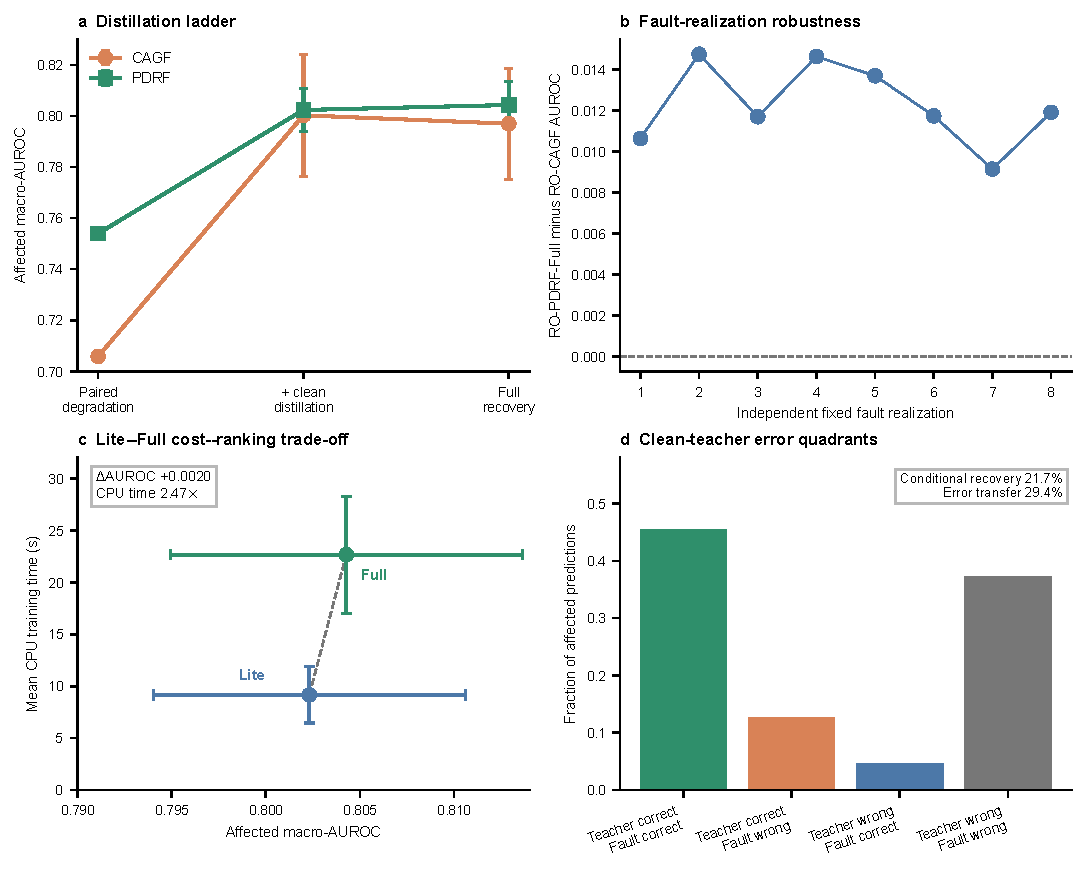
\includegraphics[width=\textwidth]{figure4_revision_controls.pdf}
\caption{\textbf{Controls for recovery mechanism, robustness and cost.} \textbf{a}, Paired degradation, clean-view distillation and the complete recovery objective for bounded and gated fusion; error bars are standard deviations across 10 optimization seeds. \textbf{b}, RO-PDRF-Full--RO-CAGF affected-AUROC differences across eight method-shared Gaussian fault realizations on one instrument. \textbf{c}, affected macro-AUROC versus measured CPU training time for RO-PDRF-Lite and RO-PDRF-Full; horizontal and vertical bars are seed standard deviations. The $+0.0020$ ranking difference required 2.47-fold mean training time. \textbf{d}, direct conditional audit: 21.7\% recovery when the clean teacher is correct and baseline is wrong, versus 29.4\% error transfer when the clean teacher is wrong and baseline is correct.}
\label{fig:revision-controls}
\end{figure}

\subsection{AHU direct diagnosis exposed a negative task boundary}

The chronological air-handling-unit tests contained 37,831 untouched future-time records, including 2,069 expert-annotated temperature-sensor faults. Because the target is the fault itself and no independent downstream state is available, this experiment cannot test whether suppressing that sensor recovers another prediction. Early fusion exceeded bounded recovery in all 15 building--seed pairs (mean AUROC difference $-0.0341$ for bounded recovery, $P<0.001$), and leave-one-building-out bounded recovery collapsed to $0.298\pm0.005$ in the hospital. The operational data therefore establish a direct-diagnosis and transfer boundary, not downstream recovery validation; complete subtype, shift, adaptation and risk analyses remain in the Supplementary Information.

\subsection{Probability quality and aggregation remained deployment limitations}

Recovery improved bounded-model probability quality without matching the recovery gate. All values in this comparison use temperatures fitted on the calibration split. On affected observations, RO-PDRF-Full NLL and ECE were 2.650 and 0.342, compared with 3.085 and 0.369 for PDRF but 2.071 and 0.275 for RO-CAGF. RO-PDRF-EMA reduced the bounded model's values to 2.413 and 0.321, whereas increasing the Brier coefficient fourfold gave 2.681 and 0.342. RO-AT-GATE achieved lower NLL and ECE (1.826 and 0.210) but lower affected AUROC (0.784). Thus no tested model dominated both class ranking and probability quality. Classwise diagrams confirmed larger average one-versus-rest calibration error for the original bounded ensemble (0.100 versus 0.072). Calibration diagrams, Brier scores, temperature sensitivity and the optional-quality-metadata failure audit remain in the Supplementary Information.

Equal-probability aggregation gave overall AUROC 0.8512 for RO-PDRF-Full and 0.8510 for RO-CAGF; their difference was 0.0002 with a 5,000-resample interval from $-0.0039$ to 0.0044. On affected rows, however, RO-PDRF-Full ensemble AUROC was 0.8186 versus 0.8368 for RO-CAGF, a difference of $-0.0181$ ($-0.0260$ to $-0.0101$). Affected NLL was also worse (2.019 versus 1.411), and RO-PDRF-Full members were less diverse (pairwise disagreement 0.181 versus 0.335). Logit averaging further reduced affected AUROC to 0.813 for RO-PDRF-Full and 0.832 for RO-CAGF and increased both NLL values. Confidence-based abstention did not reverse the ordering: at 20\% coverage, affected-row classification risk was 0.125 for RO-PDRF-Full and 0.093 for RO-CAGF, and Full remained worse at every evaluated coverage. Recovery of the complete bounded model therefore does not solve affected-row probability aggregation, calibration or selective prediction.

The discrimination--calibration audit (Fig.~\ref{fig:pareto-teacher}) makes this trade-off explicit. RO-AT-GATE had the lowest ECE but lower AUROC; QMF-PD improved substantially within the official-rule-aligned sensor-group adaptation but was dominated by RO-CAGF on these two mean metrics; and the explicitly named Lite, Full and EMA variants occupied a higher-ranking, higher-ECE region. Teacher-error controls changed recovery and transfer rates without producing a rule that isolated negative transfer. Model choice therefore depends on whether ranking, probability quality or conservative recovery supervision is operationally primary.

\begin{figure}[ht]
\centering
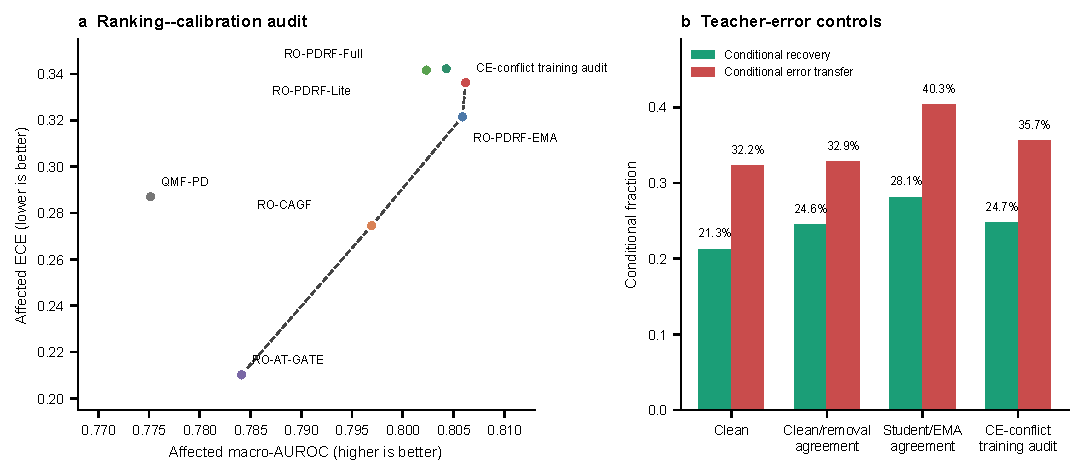
\includegraphics[width=\textwidth]{figure5_pareto_teacher.pdf}
\caption{\textbf{Ranking--calibration and teacher-error audit.} \textbf{a}, affected-subset macro-AUROC versus 15-bin expected calibration error after per-seed temperature scaling. A mean is non-dominated when no other tested mean has AUROC at least as high and ECE at most as low, with at least one strict inequality; the dashed line joins such means. \textbf{b}, conditional recovery and error transfer for ordinary clean teaching, CRA, ECA and the CE-conflict training audit. The last control is label-assisted and training-only; it is not observable at test time. Fractions are paired prediction-level audit quantities, not independent-device rates.}
\label{fig:pareto-teacher}
\end{figure}
\FloatBarrier

\subsection{Bounded fusion reduced model cost but not every memory component}

For four chemical sensor groups, PDRF used 19,740 parameters and 38,528 counted inference FLOPs, compared with 26,588 parameters and 52,224 FLOPs for CAGF. At 16 groups, the corresponding counts were 78,960 versus 106,160 parameters and 154,112 versus 208,896 FLOPs. Both scaled approximately linearly with group count. PDRF had lower model-state memory but a slightly larger counted forward-activation footprint at 16 groups (7.44 versus 6.69 KiB), so parameter efficiency is not presented as universal peak-memory superiority. Across the clean-distillation runs, maximum pre-clipping gradient norms were 0.54 for PDRF and 0.77 for CAGF; no exploding-gradient event reached the clipping threshold of 5. Complete curves and scaling data are reported in the Supplementary Information.

\section{Discussion}

The strict estimand changes the central interpretation. Clean-to-faulted prediction distillation, an established consistency-training mechanism, accounts for most of the recovery gain, and that gain increases slightly after rows without an applied fault are removed. Its value here is the recovery formulation, controlled paired-degradation protocol and explicit negative-transfer audit, not a new distillation divergence. RO-PDRF-Lite remains the efficient unconditional default because it retains nearly all affected-ranking performance with less than half the measured training time of Full. RO-PDRF-Full is the mechanistic endpoint, and SR-PDRF-Safe is the conservative deployment layer when protecting correct base decisions is more important than accepting every possible recovery. The bounded model also outperformed a stronger multi-expert router in the four-mechanism audit, but its strict Gaussian difference from the recovery-matched gate was unresolved and reversed after fixed-ensemble probability averaging. The evidence supports constrained efficiency and environment-dependent competitiveness, not universal architectural superiority.

The prediction-level audit explains both why recovery supervision matters and where it fails. In the eight-realization conditional analysis used in Fig.~\ref{fig:revision-controls}, RO-PDRF-Full recovered 21.7\% of eligible predictions when its clean teacher was correct, but transferred error in 29.4\% when that teacher was wrong. Affected-group weights usually decreased, yet suppression cannot create missing class information or reconcile incompatible logits. Hard confidence, continuous weighting, teacher agreement and label-assisted training conflict did not identify this route reliably. The multivariable selector instead learns when to accept recovery from held-out calibration interventions. Its Safe rule prevented 90.0\% of observed negative-transfer opportunities, but retained only 17.9\% of corrections and required multiple inference passes. This is a concrete risk-control result, not a solution to teacher error: selector transport remains untested for natural faults, new devices and fault mechanisms absent from calibration. RO-PDRF-EMA reduced affected NLL and ECE across all four controlled mechanisms while its crossed-factor AUROC interval included zero. None of these objectives makes the bounded operational response a physical health variable.

The hydraulic rig supplies native component-condition targets that remain meaningful after pressure or vibration sensors are corrupted, but the stricter split changes its evidential role. The mean bounded-gate difference fell from $+0.044$ under random stratification to $+0.015$ under guarded blocks, and the hierarchical interval crossed zero. This sensitivity is consistent with adjacent-cycle similarity and prevents the original condition-level result from serving as independent architecture confirmation. The chemical multi-realization audit provides stronger robustness evidence for repeated corruption, but it too remains within one instrument.

The AHU data answer a different question. Their native label is the sensor fault itself, and no independent downstream state is available. Direct diagnosis rewards preservation of the anomalous signature that recovery may suppress. Stronger EF-PD and histogram gradient boosting (HGB) results are therefore a substantive negative boundary, not an inconvenient failed validation. Creating a downstream target from the same fault label would be circular; resolving this boundary requires a dataset that jointly records sensor faults and an independent control, energy, comfort or component outcome.

Cross-building AHU results further separate task mismatch from domain shift. The bounded recovery model's hospital ordering reversed, while EF-PD transferred almost perfectly. Hospital feature, class-prior and subtype shifts are large, but simple target normalization and CORAL did not repair the bounded model, and GroupDRO did not improve an already strong EF-PD. This architecture-specific contrast argues against attributing every failure to a single scalar distance. A useful next step is a pre-registered multi-building study with target-free model selection, representation-level invariance and sufficient examples of each fault subtype.

Four deployment boundaries remain. First, 63.6\% saturation of the bounded operational response prevents interval-scale interpretation. Second, wrong clean teachers can propagate errors; the fallback reduces this route only under a calibration distribution that contains representative controlled faults. Third, equal-probability and logit-averaged RO-PDRF-Full ensembles remained inferior on affected-row probability quality, classwise calibration and selective risk. Fourth, optional quality metadata help only when trustworthy and create a new failure route when systematically misleading. The model should therefore expose the bounded response as an operational control signal, validate any external quality channel and retain abstention or calibrated fallback logic rather than presenting a calibrated device-health estimate.

The study is limited by controlled feature corruptions, one chemical instrument, one hydraulic rig, residual within-condition similarity after blocked splitting, rare AHU supply-air faults and expert/rule-based rather than maintenance-confirmed AHU labels. The eight chemical fault realizations vary corruption draws but not hardware; the four fault mechanisms are not a large top-level sample; and the eight hydraulic task--fault conditions are variants from one platform rather than devices. The selector is calibrated with the same four mechanism families used in its test audit, although its realizations and observations are disjoint, so its transport to unanticipated natural failures is unknown. The descriptive non-inferiority margin is post hoc, and the transfer/adaptation audit is exploratory. The method was developed in stages: the final upgrade protocol was frozen before its formal rerun, but repeated inspection of related outcomes during earlier revisions creates researcher-level adaptive-development risk that seed intervals cannot capture. Independent prospective replication is therefore required. Current evidence cannot support device-independent, multi-device field-recovery or maintenance-confirmed recovery claims. Those claims require prospective data from multiple devices with adjudicated sensor faults and an independent downstream target.

\section{Conclusion}

Clean-view recovery supervision improved fault-tolerant classification after the analysis was restricted to observations that actually received the controlled fault. The complete bounded model gained 0.0156 macro-AUROC over paired-degradation training across 10 matched fits, whereas its strict difference from a recovery-matched gate was unresolved. A stronger multi-expert router narrowed baseline concerns but did not exceed the bounded model across the four tested mechanisms. Calibration-only fallback then prevented 90.0\% of negative-transfer opportunities while retaining 17.9\% of available corrections and nearly preserving the four-mechanism ranking gain. The resulting contribution is a recovery-supervision protocol with a measurable risk--recovery control, an efficient bounded implementation and explicit estimand boundaries. It is not evidence for calibrated device health, natural-failure generalization or device-independent field recovery.

\section*{Data and code availability}

The Gas Sensor Array Drift Dataset (DOI: \url{https://doi.org/10.24432/C5RP6W}) and Condition Monitoring of Hydraulic Systems dataset (DOI: \url{https://doi.org/10.24432/C5CW21}) are available from the UCI Machine Learning Repository under CC BY 4.0. The operational AHU data are available from Figshare under CC BY 4.0 (DOI: \url{https://doi.org/10.6084/m9.figshare.27147678.v3}). The accompanying reproducibility package contains fixed seeds, explicit split-index manifests, controlled-fault definitions, processing and QMF-adaptation code, prediction-level outputs, 5,000-replicate bootstrap analyses, an environment specification, source tables and all main-table and figure scripts. No permanent software DOI is asserted in this version because an author-controlled public archive has not yet been created.

\section*{Ethics statement}

The study used public engineering datasets and controlled computer-generated sensor corruptions. It involved no human participants, personal data, animals or biological specimens; institutional ethics review was not applicable.

\section*{Author contributions}

Riyang Luo: Conceptualization, Methodology, Software, Validation, Formal analysis, Investigation, Data curation, Visualization, Writing--original draft, Writing--review and editing, and Project administration.

\section*{Acknowledgements and funding}

The author received no specific funding for this work and has no acknowledgements to declare.

\section*{Competing interests}

The author declares no competing interests.

\bibliographystyle{unsrtnat}
\bibliography{references}
\end{document}
